\documentclass{standalone}
\usepackage[x11names]{xcolor}
\usepackage{tikz}
\usetikzlibrary{calc}
\usetikzlibrary{arrows.meta}
\usetikzlibrary{decorations.pathmorphing}
\usetikzlibrary{decorations.pathreplacing}
\tikzset{sdot/.style = {fill, circle, inner sep = 1.5pt}}

\begin{document}
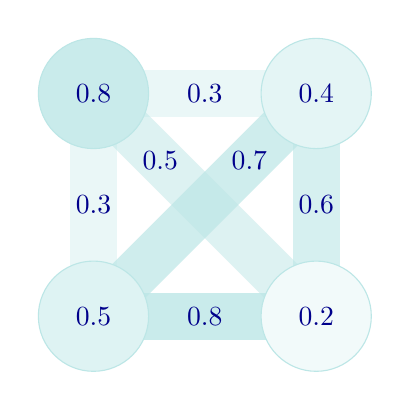
\begin{tikzpicture}
    \fill [white] (-2.25, -2.25) rectangle (2.25, 2.25);
    \foreach \i in {1, ..., 4} {
        \coordinate (\i) at (-45 + 90*\i:2);
    }
    \foreach \i\j\k\l in {1/2/0.3/0.5, 2/3/0.3/0.5, 3/4/0.8/0.5, 4/1/0.6/0.5, 1/3/0.7/0.3, 2/4/0.5/0.3} {
        \fill [DarkSlateGray3!50, opacity = \k] ($(\i)!0.3cm!90:(\j)$) -- ($(\i)!0.3cm!-90:(\j)$) -- ($(\j)!0.3cm!90:(\i)$) -- ($(\j)!0.3cm!-90:(\i)$) -- cycle;
        \node [Blue4] at ($(\i)!\l!(\j)$) {$\k$};
    }
    \foreach \i\j\k in {1/20/0.4, 2/40/0.8, 3/25/0.5, 4/10/0.2} {
        \filldraw [draw = DarkSlateGray3!50, fill = DarkSlateGray3!\j] (\i) circle (0.7);
        \node [Blue4] at (\i) {$\k$};
    }
\end{tikzpicture}
\end{document}